\chapter{Background}
\label{Background}

This chapter gives an outline of the concepts and a detailed explanation of the various technologies that will be used later in this thesis.

	\section{Containers}
	\label{Background:Containers}
	The concept of container technology uses the same model as shipping containers in transportation. The idea is that before the invention of shipping containers, manufacturers had to ship goods in a variety of fashions which included ships, trains, airplanes, or trucks, all with different sized containers and packaging.
	With the standardization of shipping containers, products could be transported seamlessly without further preparation using different shipping methods. Before the arrival of this standard, shipping anything in volume was a complex, laborious process. The motivation behind software containers is the same. \cite[P.~1]{Kinnary2018}\\

	Instead of shipping a complete operating system (OS) and the software (with necessary dependencies), we pack our code and dependencies into an image that can run anywhere. Furthermore,  it enables the packaging of clusters of containers onto a single computer. In other words, a container consists of an entire runtime environment: an application, plus all the dependencies, libraries, and other binaries, and configuration files needed to run it, bundled into one package.
	The ability to have software code packaged in pre-built software containers means that code can be pushed to run on servers running different Linux kernels or be connected to run a distributed app in the cloud. This approach also has the advantage of speeding up the testing process and creating large, scalable cloud applications. This approach has been in software development communities for several years. It has recently gained in popularity with the growth of Linux and cloud computing. \cite[P.~2]{Kinnary2018}\\
	
	% \newpage
	\subsection{Containerization vs Virtualization}
	Linux containers and virtual machines (VMs) are both package-based computing environments that combine several IT system components and keep them isolated from the rest of the system. Their main distinguishing features are scalability and portability. Containers are usually measured in megabytes, whereas VMs in gigabytes.
	\cite{containersRedHat}
	\begin{figure}[H]
		\centering
		% \input{"Bilder/tikz/Grundlagen/docker-types-of-mounts.tex"}
		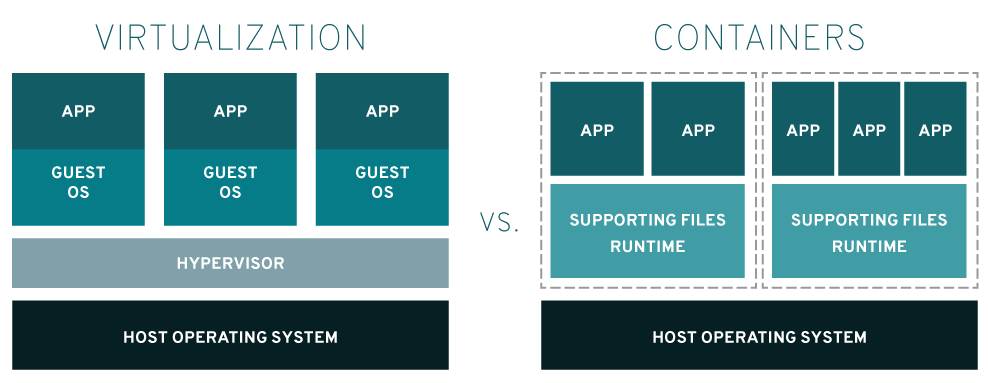
\includegraphics[width=0.9\textwidth]{"Bilder/virtualization-vs-containers_transparent.png"}
		\caption{Differences between Virtualization and Containerization \cite{containersRedHat}}
		\label{fig:Background:Containers:Containers vs VMs}					
	\end{figure}

	\paragraph*{Containerization} is an alternative to standard virtualization that encapsulates an application in a container with its executing environment.
	Containers hold an application and everything it needs to run. Everything within a container is maintained on an image—a code-based file that includes all libraries and dependencies. These files are similar to a Linux distribution installation. An image comes with RPM packages and configuration files. Containers are so small compared to VMs, there are usually hundreds of them loosely coupled together.\cite{containersRedHat}
	
	\paragraph*{Virtualization} is a way of sharing a single physical instance of a resource or an application to multiple organizations and clients. It utilizes software called a hypervisor that separates resources from their physical devices. It enables the partitioning of the resources and assigned to individual VMs. When a user issues a VM instruction that requires additional resources from the physical environment, the hypervisor sends the request to the physical system and saves the changes. VMs look and act like physical servers, which can multiply the drawbacks of application dependencies and large OS footprints—a footprint that's often not required to run a single app or microservice.\cite{containersRedHat} \\

	Table \ref{tab:container_vs_vms} illustrates the key differences between the above two approaches concerning package-based computing environments.
	\begin{table}[H]
        \centering
		\rowcolors{1}{}{gray!25}
        \begin{tabular}{{p{3cm}|p{5cm}|p{6cm}}}
            \toprule
            Parameters & Virtualization & Containerization\\
            \midrule
            Isolation & Provides complete isolation from the host operating system and the other VMs & Provides lightweight isolation from the host and other containers, but doesn’t provide a strict security boundary as a VM \\
            Operating System & Runs a complete operating system including the kernel, thus requiring more system resources such as CPU, memory, and storage & Runs the user-mode portion of an operating system, and can be customized to include just the required services for your app utilizing fewer system resources \\
            Compatibility & Runs just about any operating system inside the virtual machine & Runs on the same operating system version as the host\\
            Deployment  & Deploys individual VMs by using Hypervisor & Deploys single container by using Docker or deploy multiple containers by using an orchestrator such as Kubernetes\\
            Persistent storage  & Uses a Virtual Hard Disk (VHD) for local storage for a single VM or a Server Message Block (SMB) file share for storage shared by multiple servers & Uses local disks for local storage for a single node or SMB for storage shared by multiple nodes or servers\\
            Networking  & Uses virtual network adapters & Uses an isolated view of a virtual network adapter. Thus, providing a little less virtualization\\
            Startup time & They take few minutes to boot up & They can boot up in few seconds \\
            \bottomrule
        \end{tabular}
		\caption{Differences between Virtualization and Containerization \cite{containers-vs-vms-Baeldung}}
		\label{tab:container_vs_vms}
    \end{table}

	The use of containers can decrease the required time for developing, testing, and deploying applications. It makes testing and fault detection less complex as there is no difference between running your application on a test environment and in production. It provides a cost-effective solution and can help reduce operational and development expenses. In most use-cases, container-based virtualization offers several advantages over traditional Virtual Machine based virtualization.

	\section{Docker}
	\label{Grundlagen:Docker}
	\textit{Docker is a person who works at a port whose job is to load goods onto and off container ships.} \cite{docker-definition-english}

	Software Docker essentially does the same in the software context. Docker is a collection of open-source tools that quickly wraps up any application and all its unique dependencies in a lightweight, portable, self-sufficient container that can run virtually anywhere on any infrastructure.\cite{docker-definition}
	Docker was launched as an open-source project by dotCloud, Inc. in
	2013. it relies heavily on namespaces and cgroups to provide resource isolation and to package an application along with its dependencies. This bundling of dependencies into one package allows an application to run across different platforms and still support a level of portability. This provides flexibility to developers to develop in the desired language and platform. It has drawn a lot of interest in recent years.\cite[P.~10]{Kinnary2018}

	Docker consists of several parts. The following section gives an overview of the main components of Docker.


		\subsection{The Docker Runtime and Orchestration Engine (Docker Engine)} 
		\label{Grundlagen:Docker:Docker Engine}
		The Docker engine is the software for the infrastructure that runs and orchestrates containers. All other Docker, Inc. and third-party products connect to and develop around the Docker Engine. It provides a workflow for building and managing the application stack. It builds and runs containers using other Docker components and services. It consists of the Docker daemon; a REST API that specifies the interfaces that programs can use to communicate with the daemon; and the CLI, the command-line interface that communicates with the Docker daemon via the API. Docker Engine creates and runs the Docker container from the Docker image file.\\
		\\
		Following Diagramm illustrates the Docker System Architecture.
		\begin{figure}[H]
			\centering
			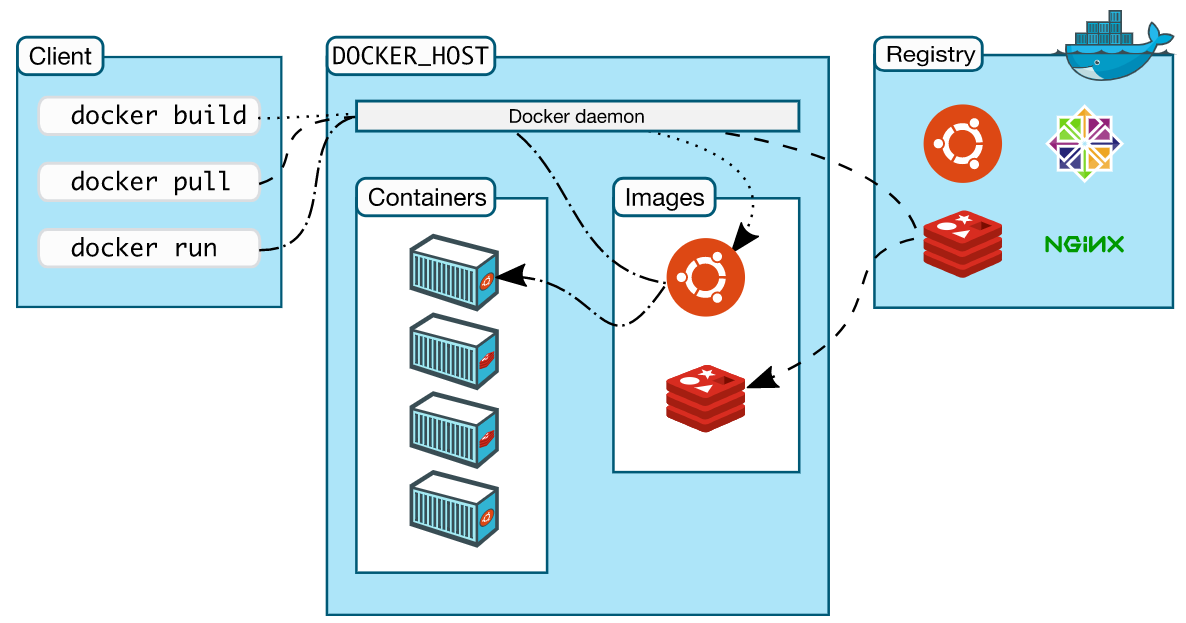
\includegraphics[width=0.9\textwidth]{"Bilder/DockerArchitecture.png"}
			\caption{Docker System Architecture \cite{dockerOverwiew}}
			\label{fig:Background:DockerEngine:Architecture}					
		\end{figure}

		\paragraph{Docker daemon (dockerd)}  is a server process that runs
		in the background. It continuously listens to the REST API interface
		and listens for incoming requests and manages Docker objects (images, containers, networks, and volumes).  A daemon also has the ability to communicate with other daemons to manage Docker services.\cite{dockerOverwiew}

		\paragraph{Docker client} represents the primary means for most users to interface with Docker. The commands run through the command-line interface are sent to the Docker daemon through the Docker API interface. The Docker daemon(dockerd) then executes these commands. The Docker client has the ability to connect with multiple Docker daemons.\cite[P.~32]{Kinnary2018}
		
		\paragraph{Docker registry} The images created by the Docker daemon are stored in the Docker registry. Docker looks for images in the Docker Hub by default, but it is possible to have a self hosted private registry. Docker Hub is a public registry and is freely accessible.\cite[P.~33]{Kinnary2018}
			
		\subsection{Docker Objects}
		\label{Grundlagen:Docker:Docker Objects}
		\paragraph{Images}
		A Docker image is a read-only file system that contains instructions to create a container in which an application can run. In most cases, a Docker Image is based on another image and is customized. You can either use existing images published in public repositories such as Docker Hub or Create your image.
		A Dockerfile is used to create a Docker image. A Dockerfile contains simple instructions that can be understood by the Docker daemon to	create the image and run it. Docker images are layers that correspond to each instruction in the Dockerfile. Part of what makes a Docker image super easy is that when you change a part of the Dockerfile, only that layer is changed, and not the entire image.

		\paragraph{Containers}
		A Docker container is an instance of an image. An image runs inside a container. You can manage a container with the stop, start, and delete commands to manage it. Multiple containers can be connected over a network. They can be connected to the memory, and they can also communicate with each other. Containers are much more lightweight than VMs because their startup times are very fast. To create a container, in addition to the container's configuration and settings, you also create an image Configuration and settings an image is created. When a container is deleted everything related to the container is also deleted, including state and memory.

		\paragraph{Services}
		In a distributed application, different functionalities of the app provide different services. For example, if you are building an application that suggestions based on keywords that the user enters, you might want to have A front-end service that takes the word and sends it to the service that will Verifies the legitimacy of the word. This in turn could be sent to another service that runs an algorithm to generate the suggestions, etc., which are then returned to the service. These are all different services on different Docker containers, sitting Sit behind different Docker daemons. These Docker daemons are all connected over the network and interact with each other.
		All these services work together as a swarm, managed by different Managers and workers to manage. Each swarm contains a Docker daemon. These Daemons communicate with each other using the Docker API. A Docker Compose YAML file is used to get all these services running together. together to get them running. 

		\paragraph{Networks}

		\paragraph{Volumes}
			
			
		\paragraph{Dockerfiles}
		Dockerfile is a text document that contains a set of instructions or commands for assembling an image that is understood by the build engine. The build engine understands. The Dockerfile defines what goes into the environment inside your container. Accessing resources, mapping volumes, passing arguments, copying files that need to be inside your container are defined in this file. According to Dockerfile created, you need to build it to create the image of the container. Create container image. The image is just a snapshot of all the executed statements in the Dockerfile. Once this application image is created, you can expect that it will run on any machine that uses the same kernel. 
		
		\paragraph{Docker-Compose}
		Docker Compose is the tool for running multi-container Docker applications. It is essentially a YAML file that can be thought of as a Compose of multiple Dockerfile containers, which can be used to put commands into a single file. This Docker Compose YAML file contains configurations of multiple services. Then, with a single command, you can run all services to run in Docker containers at the same time.
		Docker Compose can be used to create a microservices architecture and link the containers together, or it can be used for a single service. In addition, Docker Compose can create images, scale containers, and re-run containers that have been stopped. All of these functions are part of Docker. Docker-compose is just a higher-level abstraction of container execution commands. Everything that a compose file can do, can likewise be performed with simple Docker commands, except that this requires more memory and additional overhead to execute any additional commands, to connect to the network, etc. . Docker-compose helps to simplify this process.
				
	\section{Industrial Edge}
	\label{Grundlagen:IndustrialEdge}
		
	Industrial Edge is a development from Siemens that makes it possible to analyze data generated in various industrial processes on the device itself. It combines local engineering with cloud engineering.\cite{siemensIndustrialEdge}

	This eliminates unnecessary data transport between the end device and the server, only processed data is sent to the server. The processing load is in this way directed from the server towards the end device. Edge applications serve this purpose, they contain a fixed set of functions and can be accessed with the edge infrastructure on the respective end device (edge device). These apps are based on Docker technology and run one or more Docker containers in them. Figure \ref{fig:Grundlagen:IndustrialEdge:Ueberblick} shows a typical infrastructure from the top server to the end devices.

		\begin{figure}[h]
			\centering
			%\input{"Bilder/tikz/Grundlagen/industrial-edge-overwiev.tex"}
			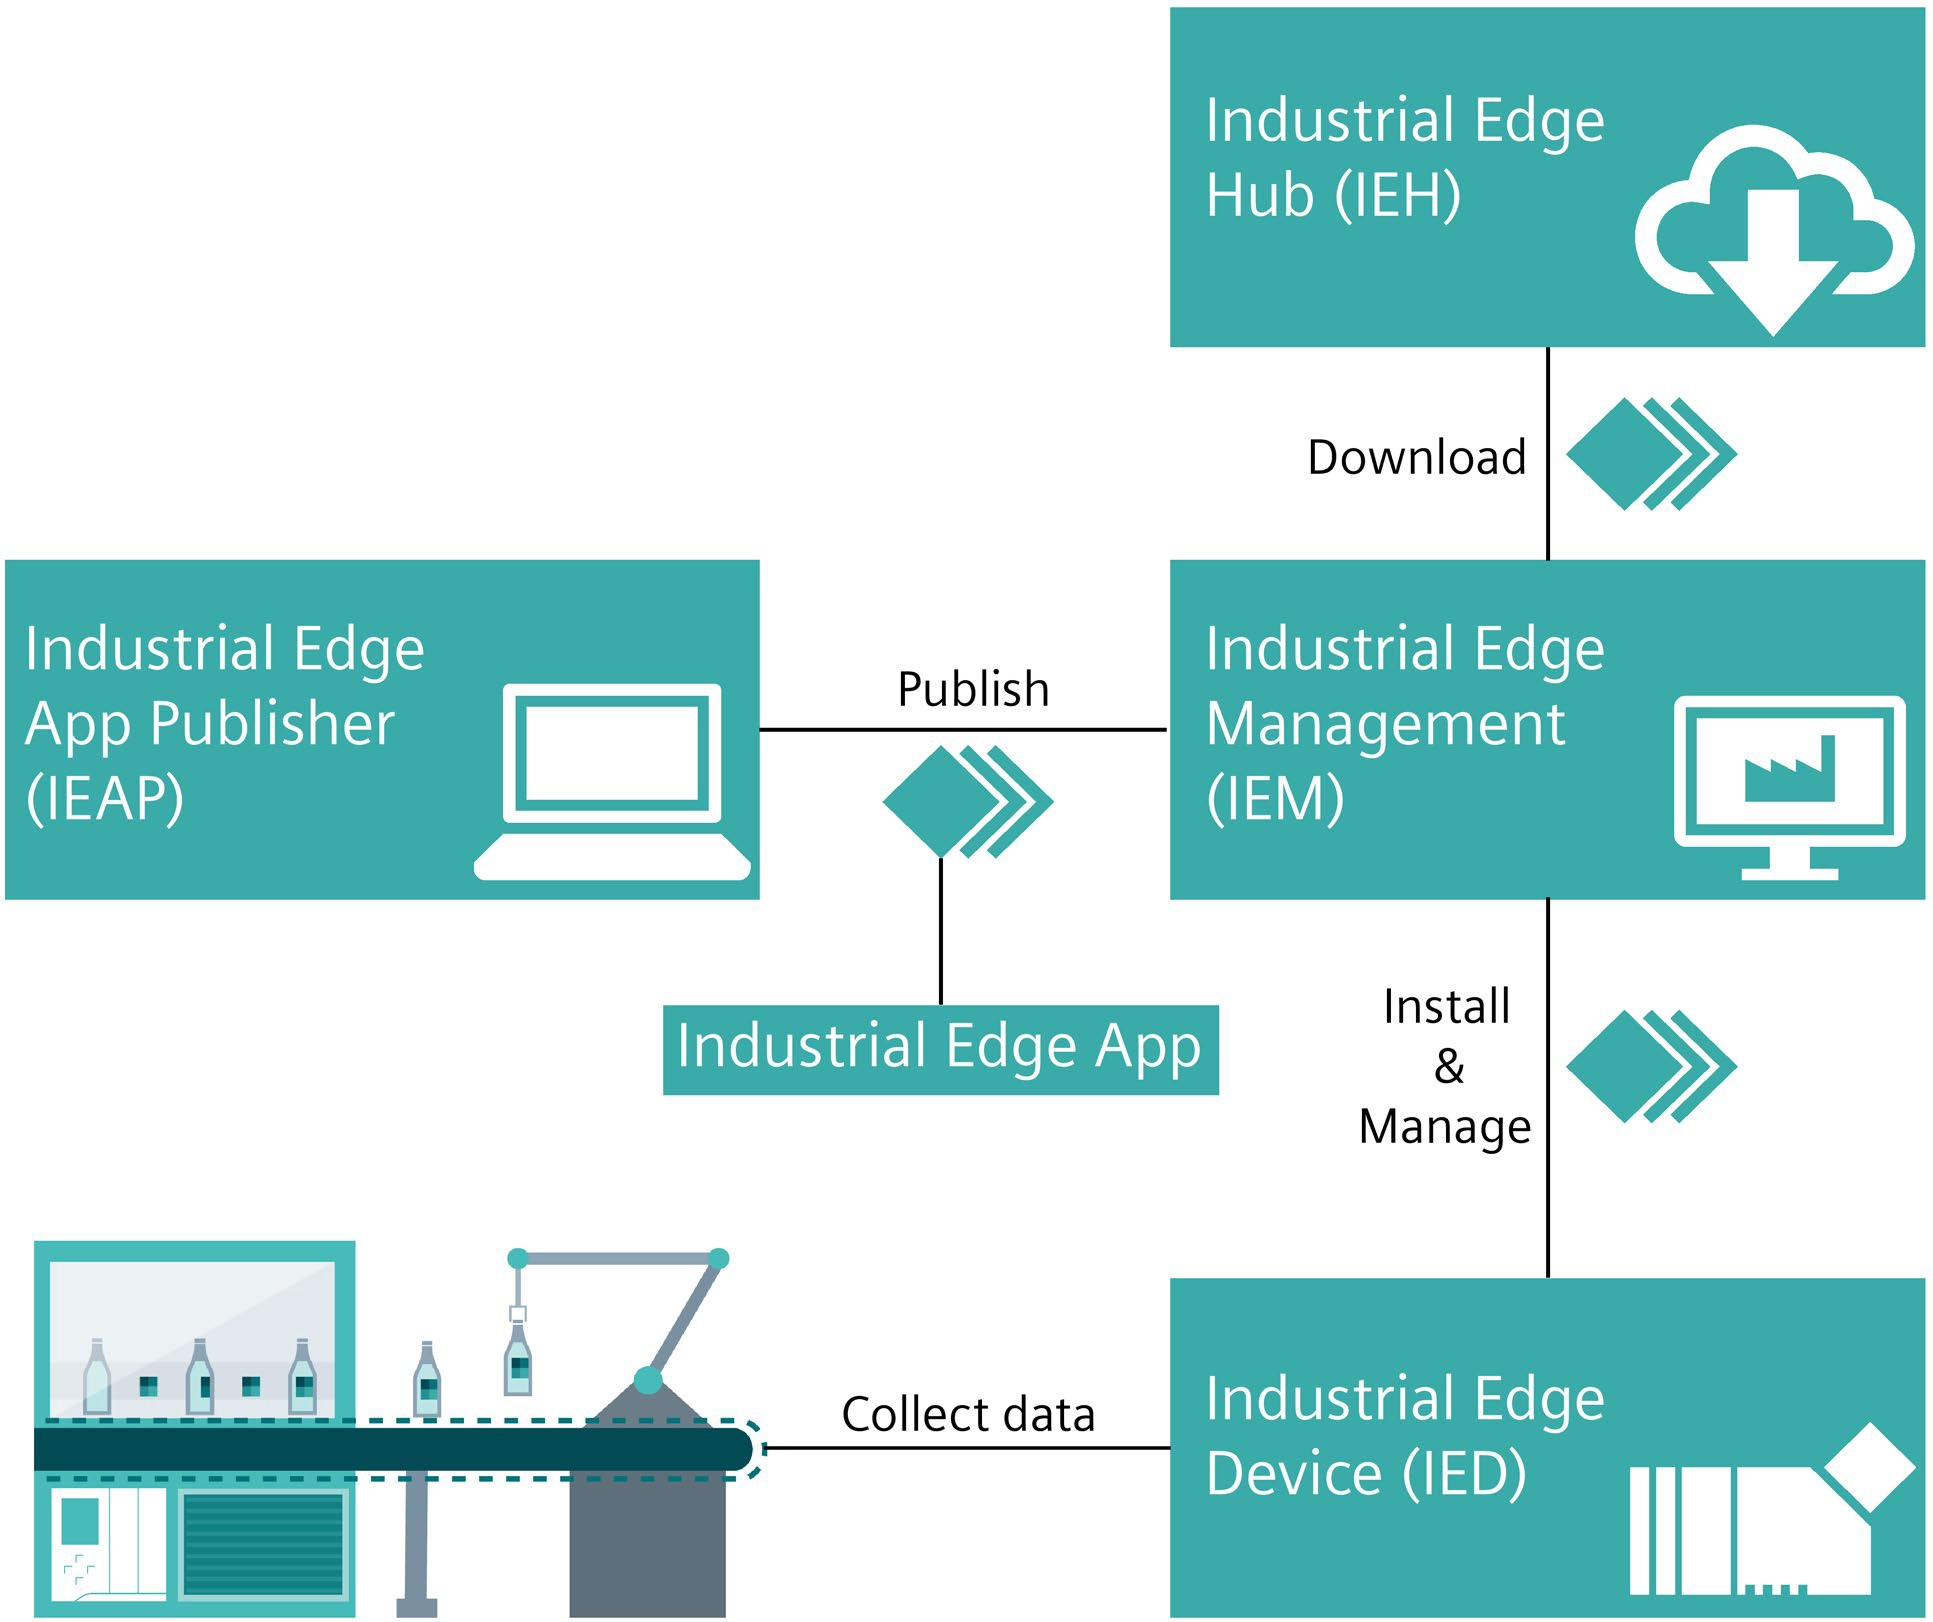
\includegraphics[width=0.70\textwidth]{"Bilder/Edge_uebersicht.jpg"}
			\caption{Industrial Edge overview \cite{siemensIEM_gettingStarted}}
			\label{fig:Grundlagen:IndustrialEdge:Ueberblick}					
		\end{figure}
	
		%- Management tool für Docker Container auf Geräten (Device)\\
		%- Graphen die das IE-Hub, IEM, Docker Device erklärt\\
			
		\paragraph{Industrial Edge Management System}
			The \gls{IEM} is a server, which can be operated independently in a local network. It allows the user to create their own server which avoids the transmission of raw sensitive data exchanged between the edge device and the IEM over the Internet.

			In addition, the end(edge) devices can be managed via this server, which includes the installation of apps and software updates and further analysis of individual apps. A self-developed Application can be uploaded to the IEM, which in turn can distribute it to the edge devices.\cite{siemensIndustrialEdge}

		\paragraph{Industrial Edge Hub}
			The \gls{IEH} 
			is the top server-level Application hub provided by Siemens. On this platform, Siemens offers applications developed in-house. These can be loaded onto the IEM for a license fee. Any required software packages and documentation can be downloaded from here. This streamlines the development process of custom applications including deployment, and operation on desired IEM.\cite{siemensIndustrialEdge}
		\paragraph{Industrial Edge App}
			An \gls{IEA} (edge app) is used for the intelligent processing of industrial automation tasks.\cite{siemensIndustrialEdge} It is a Docker-based image, which is runs on the IED. A docker-compose file acts as the top description level file, it specifies various parameters and the sequence in which the Docker images are started. The parameters include network configuration, data storage, and other application-specific configurations. It supports all Docker-compose version 2.4 settings. Modification of this docker-compose file allows configuring any Edge app, even after it has been already downloaded to an edge device. An Edge App can be downloaded to an edge device through the IEM.
	
		\paragraph{Edge Device}
		Edge devices are required in order to run individual edge apps. The edge device is a custom Linux Machine running the Industrial Edge OS. For test and simulation purposes it can also be run in a Virtual machine(VM). Edge devices can save automation data locally and retrieve it when required. In addition, edge devices can upload this data into the cloud infrastructure and retrieve it at any moment. After proper configuration and connection,  an Edge Device can be activated through IEM using an Edge Device configuration file.
			
		\paragraph{Industrial Edge Publisher}
		The Industrial Edge Publishers is a tool that converts Docker images into Edge Apps and uploads them to the IEM. It can also be used to manage, modify or delete apps that have already been created.\cite{siemensIE_App} A prerequisite for creating an app is a docker-compose file, which contains the startup parameters of a Docker container. These parameters can also be configured through a menu within the Edge Publisher.
			

	
	\section{ROS}
	\label{Grundlagen:ROS2}		
	This chapter covers the basics of the robot operating system (ROS) and all the tools necessary to create, debug, and understand robot applications. This chapter describes some high-level concepts and low-level API commands which enable developers to develop, maintain and support multi-robot applications. \\
	
	The software stack of a typical robot system requires several software tools which include hardware drivers, network modules, communication architecture, and several application-specific algorithms. ROS provides these tools in one package, which saves developers a lot of time and redundant work. ROS includes several sub-packages for robot navigation, vision, control, simulation.\\
	
	The Robot Operating System (ROS) has long been one of the most widely used middleware for robotic. The large open-source robotics community has contributed to a lot of new features since the introduction of ROS 1 in 2007, limitations of ROS1 have led to the development of ROS2.\cite{ros2Basic}\\

	\subsection{ROS2} 
	\label{Grundlagen:ROS:ROs2}
	\gls{ROS2} was launched with an improved architecture and upgraded features. It is new and various organizations and open-source communities are trying to port existing packages to ROS 2.\cite{ros2Basic} \\
	
	Table \ref{tab:ros1_vs_ros2} illustrates the key differences between ROS1 and ROS2
	\begin{table}[H]
        \centering
		\rowcolors{1}{}{gray!25}
        \begin{tabular}{{p{3cm}|p{5cm}|p{6cm}}}
            \toprule
            Parameters & ROS1 & ROS2\\
            \midrule
            Networking & Utilizes the TCPROS communication protocol & Uses DDS (Data Distribution System) for communication.\\
            ROS Master & Uses ROS Master for centralized discovery and registration. The whole communication system fails if the master fails. & Uses the distributed DDS discovery. ROS 2 provides a custom API to get all information about nodes and topics. \\
            Compatibility & ROS runs only in Ubuntu. & ROS 2 is compatible with Ubuntu, Windows 10, and OS X.\\
            Programming language  & Uses C++ 03 and Python2. & Uses C++ 11 and Python3.\\
            Build system  & ROS uses only the CMake build system and has a combined build for multiple packages via a single CMakeLists.txt file & ROS 2 offers options to use other build systems. Supports isolated independent builds for packages to better handle dependencies between packages.\\
            Default values & Data types in message files do not support default values. & Data types in message files support default values.\\
            roslaunch & roslaunch files are written in XML. & roslaunch files are written in Python which makes it more configurable and and supports conditional execution.\\
            Realtime Support & Does not support Real-time behavior. & Supports real-time responses with a suitable RTOS.\\
			\bottomrule
        \end{tabular}
		\caption{Differences between ROS1 and ROS2 \cite{ros1vsros2}}
		\label{tab:ros1_vs_ros2}
    \end{table}

	\subsection{ROS2 Structure}
	\label{Grundlagen:ROS2:ROS2_Structure}
	The key ROS2 feature is that it uses DDS (Data Distribution System) for communication. It eliminates ROS Master and utilizes distributed DDS discovery.	A set of related nodes located on the same computer are called a hub, where one or more hubs can be present on the same computer. ROS hubs are considered to have an accompanying set of bridging nodes that pass messages between ROS and ROS2.\cite*[P.7]{Koubaa2021}
	\begin{figure}[H]
		\centering
		% \input{"Bilder/tikz/Grundlagen/docker-types-of-mounts.tex"}
		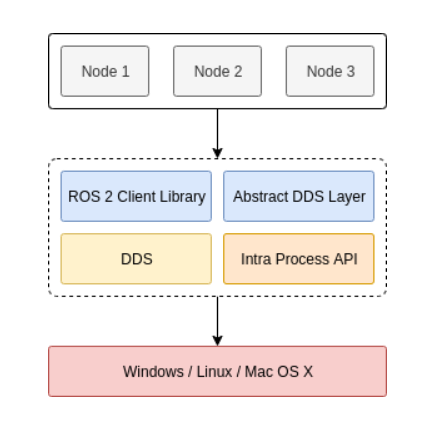
\includegraphics[width=0.5\textwidth]{"Bilder/Ros2_Architecture.png"}
		\caption{ROS2 Architecture \cite{ros1vsros2}}
		\label{fig:Background:Containers:Ros2_Architecture}					
	\end{figure}
	
		\subsection{Nachrichtentypen}
		\label{Grundlagen:ROS2:Nachrichtentypen}
			- Message (topics)\\
			- Service\\
			- Action
			
		\subsection{ROS 2-web Bridge}
		\label{Grundlagen:ROS2:2WebBridge}
			
		\subsection{roslibjs}
		\label{Grundlagen:ROS2:RosLibJS}
		
		\subsection*{Ros Lifecycle nodes}
		\label{Grundlagen:ROS2:Lifecycle}
	\section{DDS}
	\label{Grundlagen:DDS}
		- Grundlage für Kommunikation von ROS2\\
		- Realisiert die eigentliche Kommunikation\\
		- Wenn das hier geht, geht auch ROS2!
		- Verschiedene Systemanbieter, näher wird RTI und Fastrtps untersucht: https://ros.org/reps/rep-2000.html  (Beide TIER 1)
		
	
		
		
